% Chapter 4

\chapter{Substrate engagement and subunit communication} % Write in your own chapter title
\label{Chapter4}
\lhead{Chapter 4. \emph{Substrate engagement and subunit communication}} % Write in your own chapter title to set the page header


\section{Introduction}

%%-------------------------

\section{Results}

\subsection{Monitoring substrate engagement by the base unfoldase}
%fig titin concatemers and reaction schematic
%ub?
%scans
%MTO
%STO with curve fits and rate constants

%fig DATA

Data, as seen in Figure \ref{fig:titinconstructs} and Figure \ref{fig:titintablegel}.

And schematic and chemical structure in Figure \ref{fig:reactionscheme} and Figure \ref{fig:titinstructure}.

More data, as seen in Figure \ref{fig:titincarboxy}.

%\begin{table}[H]
	%\centering
%	\ra{1.3}
%	\caption[Titin concatamer molecular weights]{Titin concatamer molecular weights.}
%\begin{tabular*}{.5\linewidth}{ m{0.15\linewidth}C{0.15\linewidth} C{0.15\linewidth} }\toprule
%Construct & Number of Amino Acids & Molecular Weight (Da)\\
%\midrule
%Titin1 & 150 & 16427\\
%Titin3 & 332 & 36672\\
%Titin5 & 514 & 56933\\
%Titin10 & 977 & 108368\\
%\bottomrule
%\end{tabular*}
%\label{table:holoenzyme}
%\end{table}	


%%-------------------------
\begin{figure}[H]
\centering
\subfigure{%
	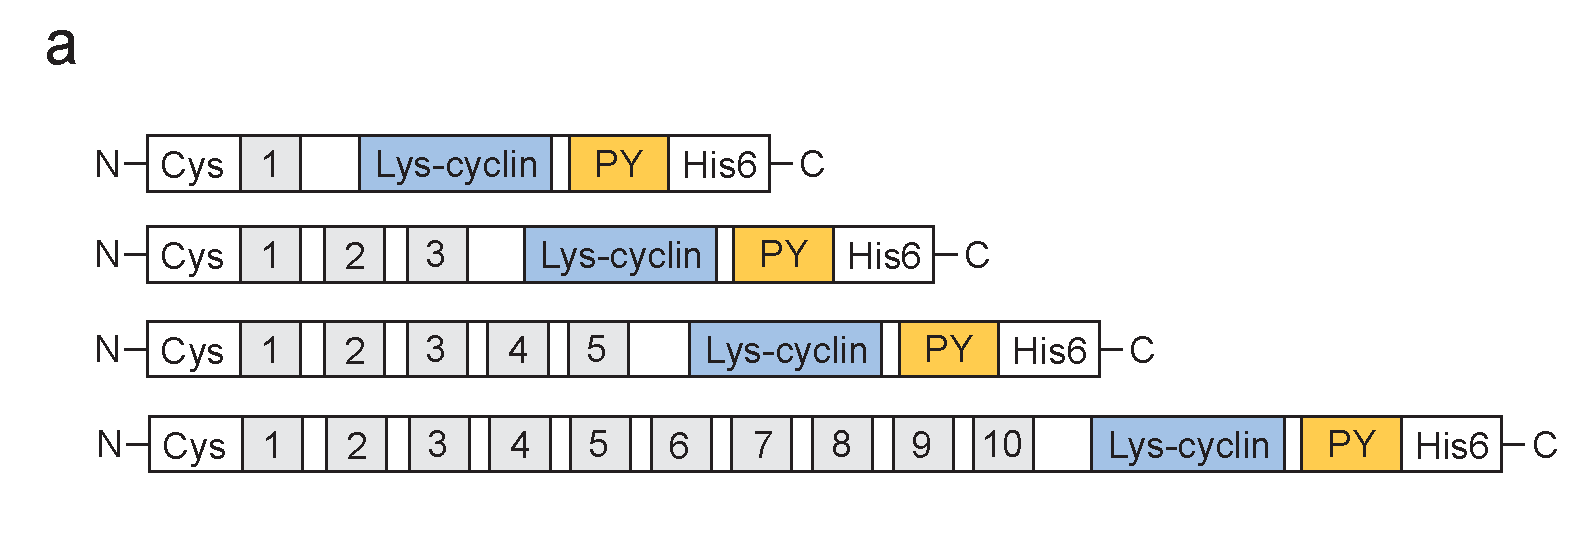
\includegraphics[scale=0.45]{titinconstructs}
	\label{fig:titinconstructs}}
\quad	
\subfigure{%
	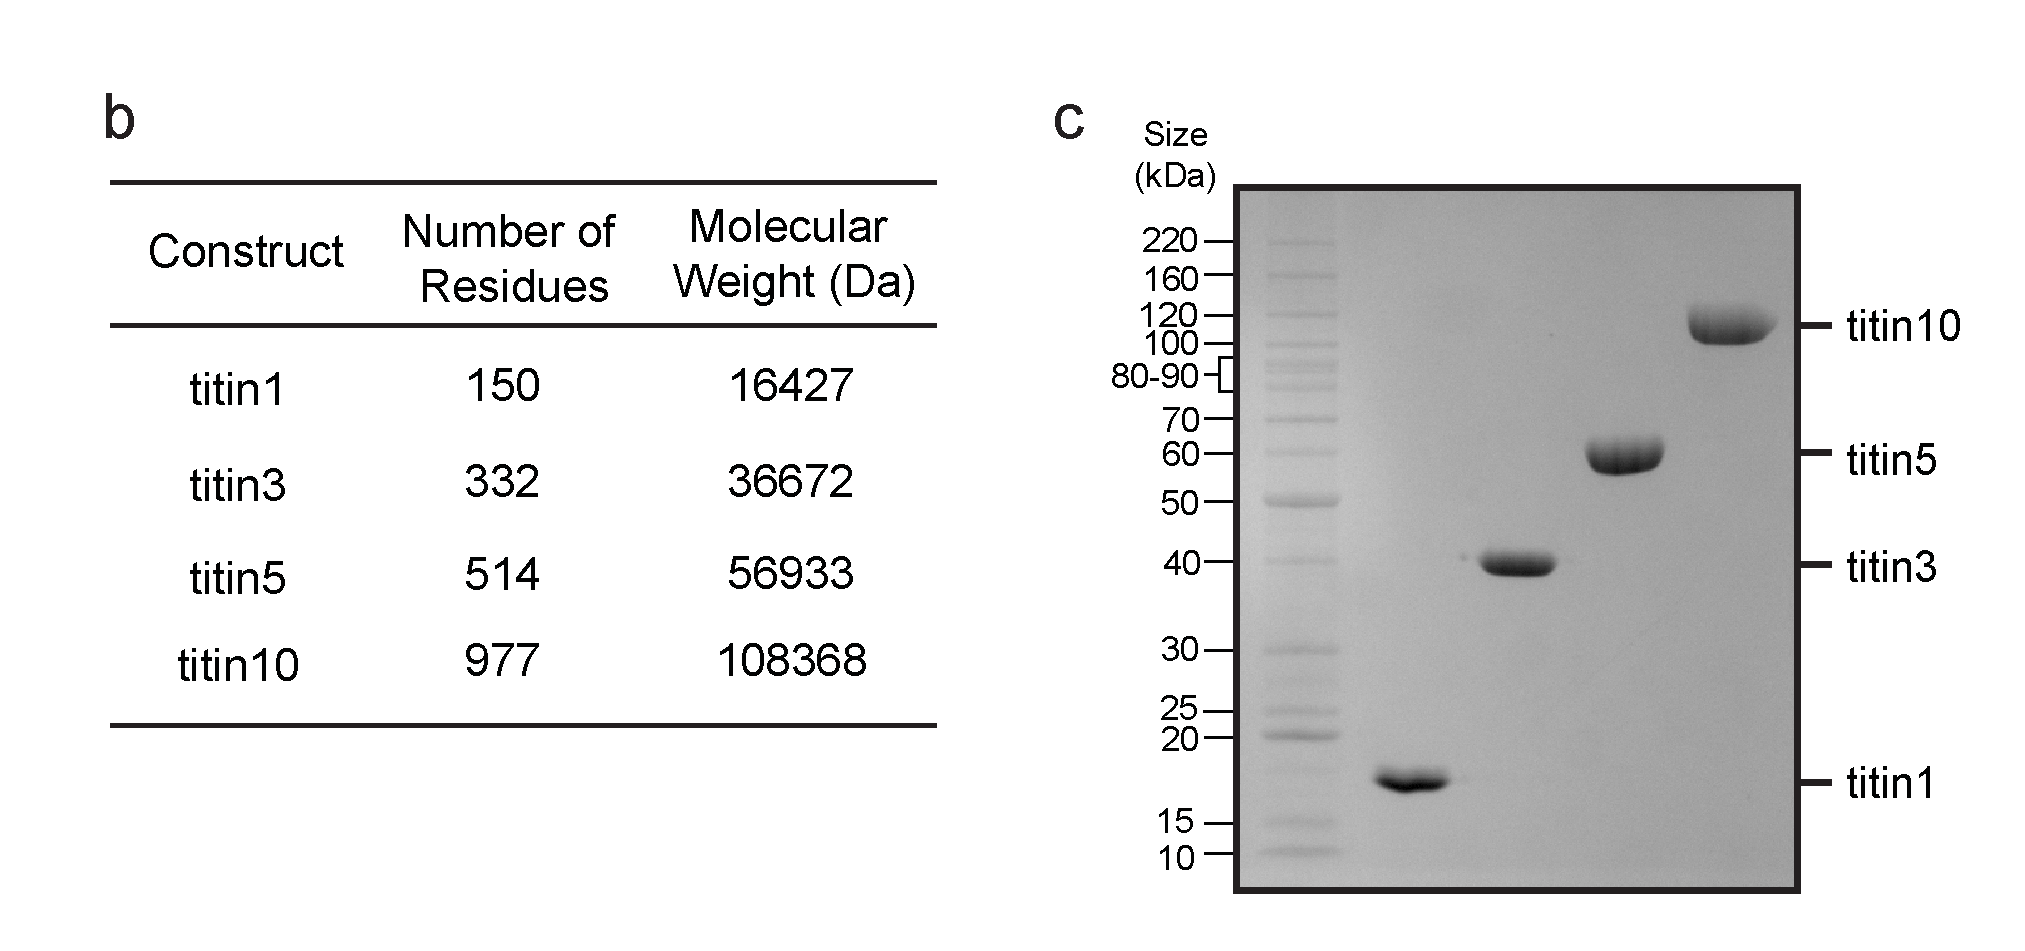
\includegraphics[scale=0.45]{titintablegel}
	\label{fig:titintablegel}}
%
\caption[Design and expression of titin concatamers]{Design and expression of titin concatamers.\par
\textbf{(a)} Predicted molecular weight for titin constructs. \textbf{(b)} Some more words.  \textbf{(c)} Some more words.
}
\label{fig:titin}
\end{figure}
%%-------------------------

%%-------------------------
\begin{figure}[H]
\centering
\subfigure{%
	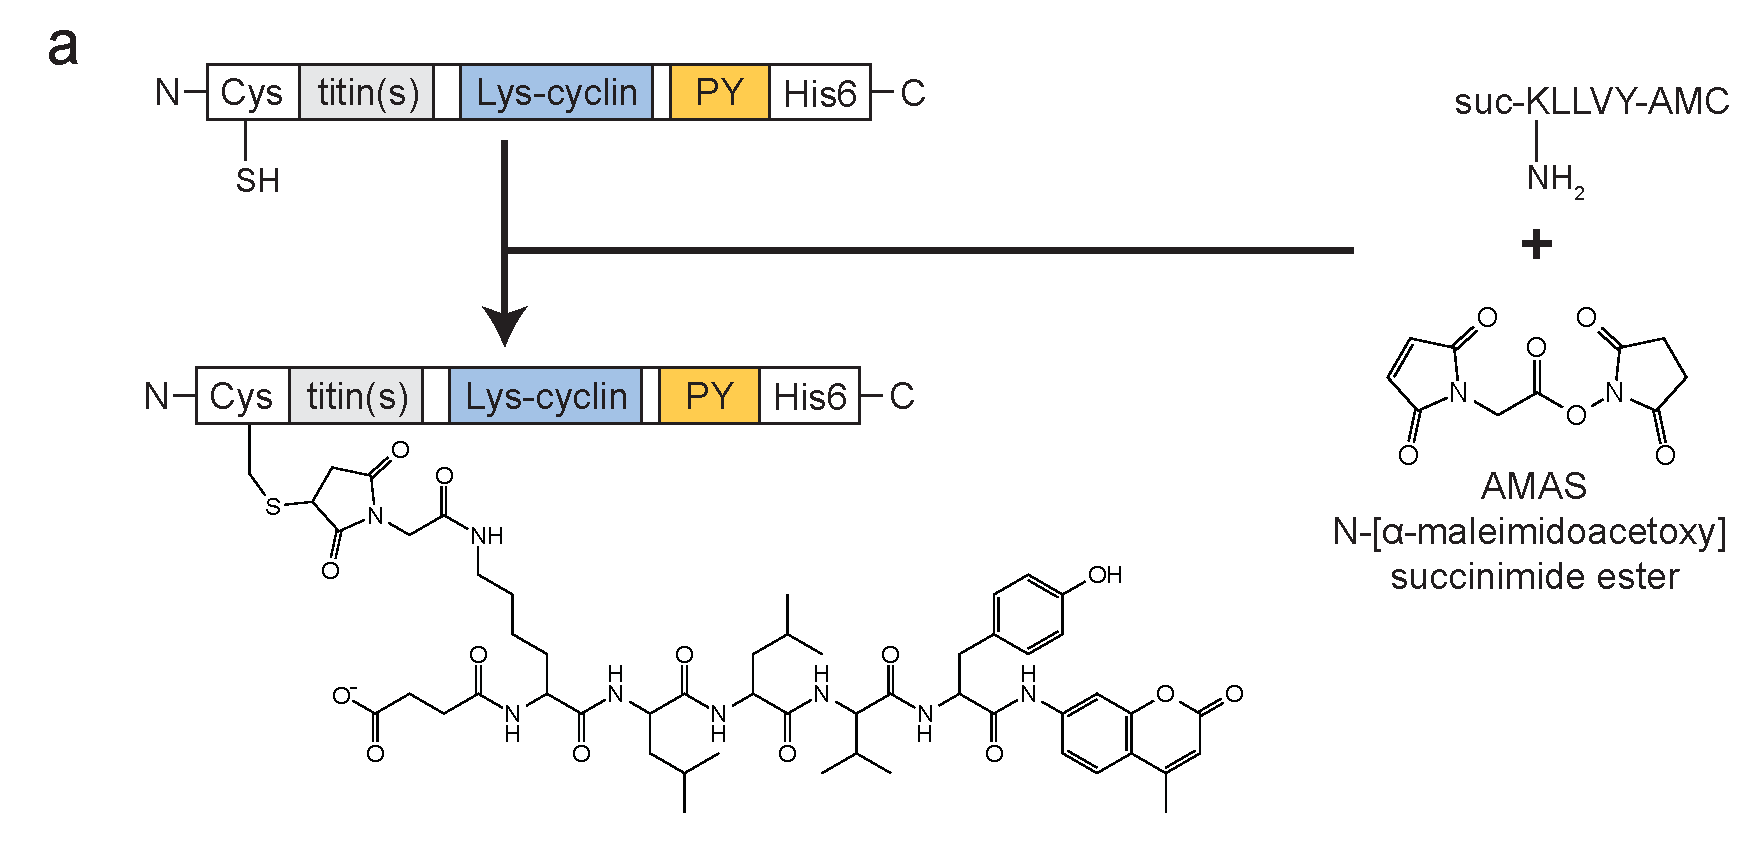
\includegraphics[scale=0.5]{titinstructure}
	\label{fig:titinstructure}}
\quad	
\subfigure{%
	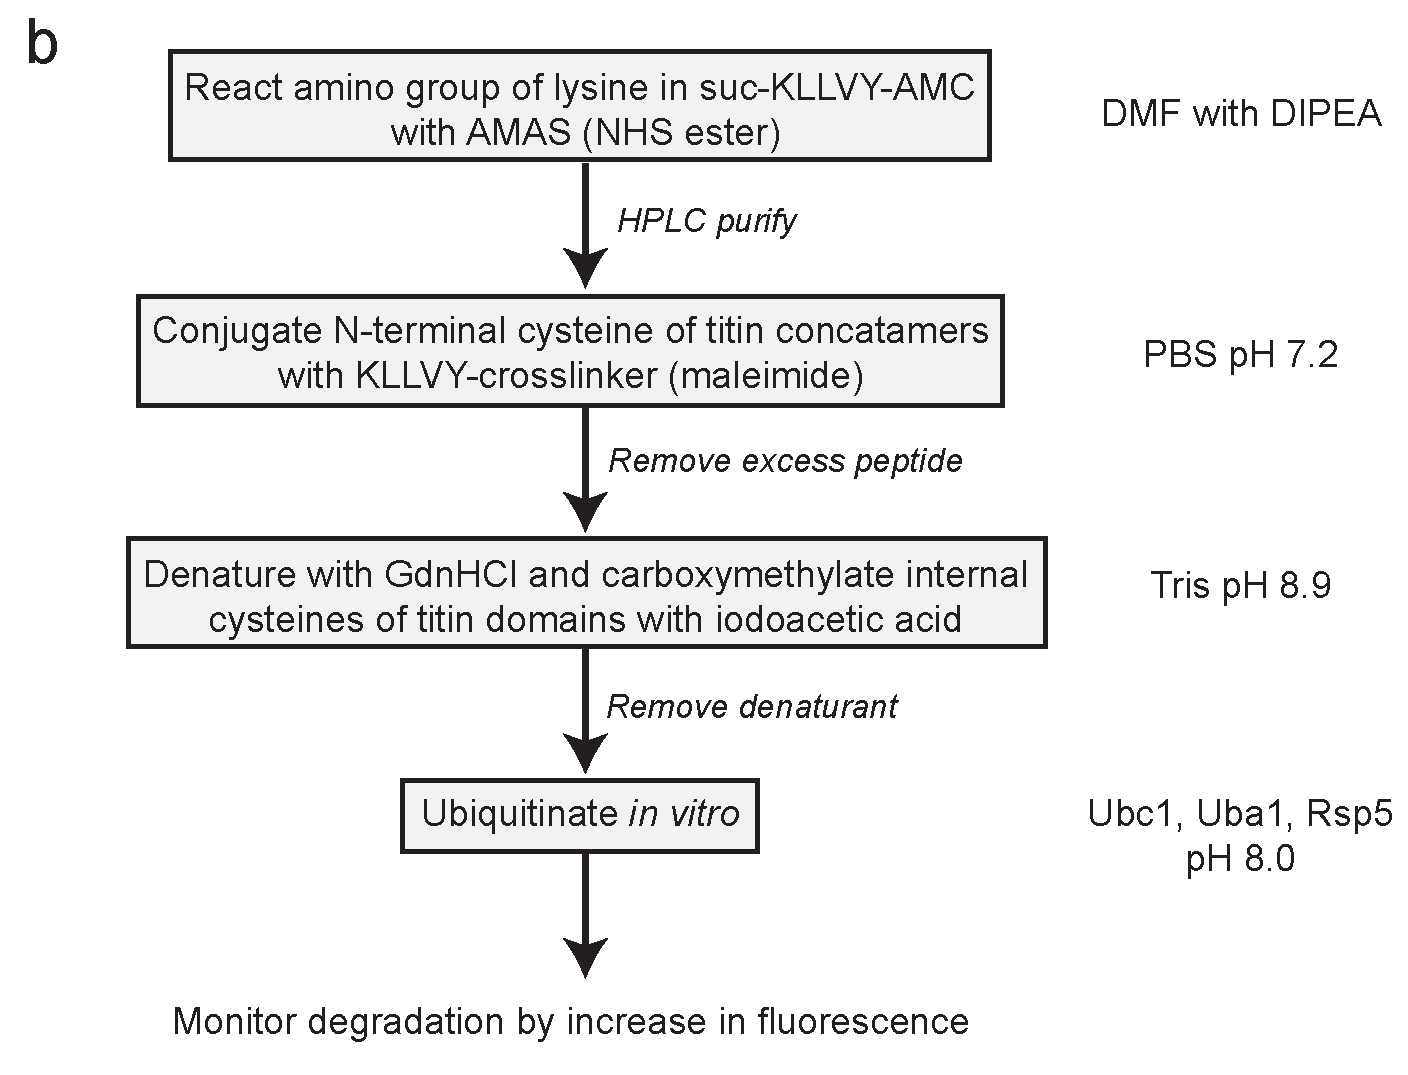
\includegraphics[scale=0.5]{reactionscheme}
	\label{fig:reactionscheme}}
%
\caption[title]{title.\par
\textbf{(a)} Predicted molecular weight for titin constructs. \textbf{(b)} Some more words.
}
\label{fig:titin}
\end{figure}
%%-------------------------

%%-------------------------
\begin{figure}[H]
\centering
\setlength{\fboxrule}{0pt}
\fbox{%
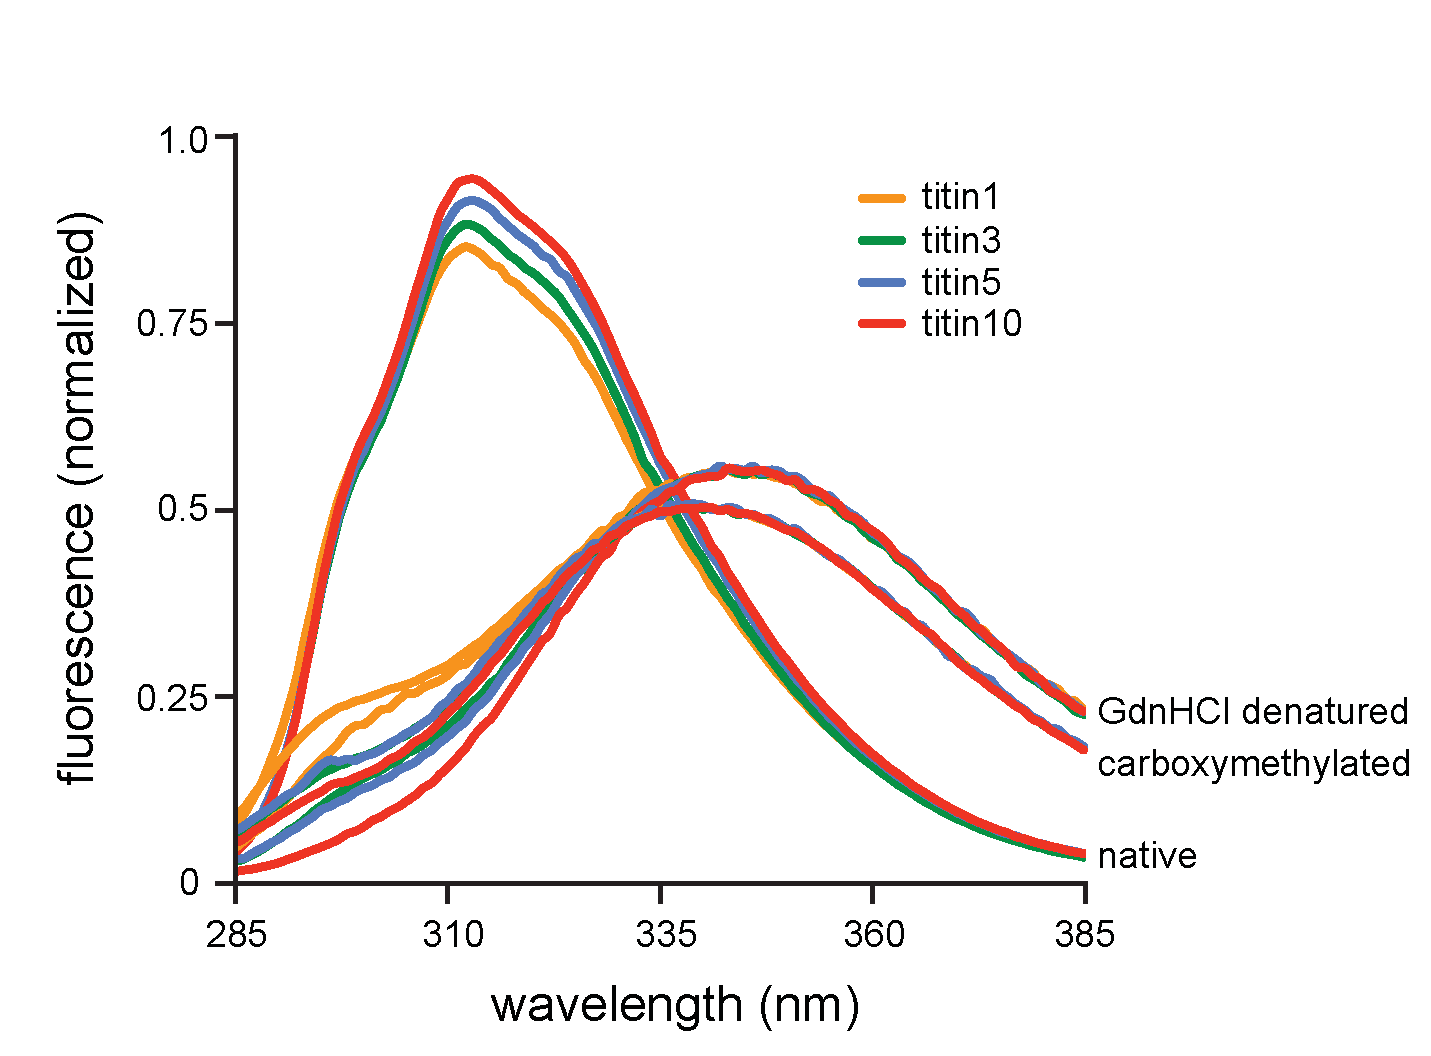
\includegraphics[width=0.9\textwidth]{trpfluor}%
}
\caption[Carboxymethylation of titin concatamers]{Carboxymethylation of titin concatamers.\par

}
\label{fig:titincarboxy}
\end{figure}
%%-------------------------




\subsection{Involvement of the arginine finger in subunit communication}
%table
	%RA, RK, EQRA?
%fig degradation bar graph



%%-------------------------

\section{Discussion}

%%-------------------------

\section{Materials and Methods}

\subsection{Cloning, expression and purification of titin concatemers}

\subsection{Labeling, carboxymethylation and ubiquitination of titin concatemers}

\subsection{Single and multiple turnover titin degradation assay}
%curve fits


%%-------------------------

